\documentclass[11pt,a4paper]{article}

\usepackage[margin=1in]{geometry}
\usepackage{mathptmx}
\usepackage{amsmath}
\usepackage{amssymb}
\usepackage{amsthm}
\usepackage{braket}
\usepackage{tikz}
\usepackage{quantikz}
\usepackage{enumitem}
\usepackage{hyperref}
\usepackage{xcolor}

\definecolor{circuitblue}{RGB}{40,80,160}

\hypersetup{
    colorlinks=true,
    linkcolor=circuitblue,
    urlcolor=circuitblue,
    citecolor=circuitblue
}

\theoremstyle{definition}
\newtheorem{definition}{Definition}[section]
\newtheorem{example}{Example}[section]

\theoremstyle{remark}
\newtheorem*{intuition}{Intuition}
\newtheorem*{keypoint}{Key Point}

\pagestyle{plain}

\setlength{\parindent}{0pt}
\setlength{\parskip}{6pt}

\begin{document}

\begin{center}
    {\LARGE \textbf{Simple Quantum Algorithms II}}\\[8pt]
    {\large QML}\\[12pt]
    \hrule
\end{center}

\vspace{12pt}
\tableofcontents
\newpage

%% ========================================================
\section{Overview}
%% ========================================================

this lecture covers the heavy hitters: quantum fourier transform (QFT), quantum phase estimation (QPE), shor's algorithm, and grover's search. these r the algorithms that actually matter for the real world --- shor's for cryptography, grover's for search, and QPE as a subroutine in basically everything.

for QML specifically, QPE shows up in quantum kernel estimation, and grover's search connects to amplitude amplification techniques used in quantum classifiers. the variational structure of QAOA (lecture 10) can be seen as a ``poor man's'' version of adiabatic evolution, which connects to QPE.

%% ========================================================
\section{The Quantum Fourier Transform}
%% ========================================================

\subsection{Classical DFT Review}

the discrete fourier transform (DFT) maps a vector $\mathbf{x} = (x_0, x_1, \ldots, x_{N-1})$ to $\mathbf{y} = (y_0, y_1, \ldots, y_{N-1})$:
\[
y_k = \frac{1}{\sqrt{N}}\sum_{j=0}^{N-1} x_j \omega^{jk}, \quad \omega = e^{2\pi i/N}
\]

classically, the FFT computes this in $O(N \log N)$ operations. quantumly, we can do it in $O(\log^2 N)$ gates --- exponentially faster. but there's a catch we'll get to.

\subsection{QFT Definition}

\begin{definition}
the \textbf{quantum fourier transform} on $N = 2^n$ basis states:
\[
\boxed{\text{QFT}\ket{j} = \frac{1}{\sqrt{N}}\sum_{k=0}^{N-1} e^{2\pi ijk/N}\ket{k}}
\]
\end{definition}

equivalently, the QFT can be written in product form:
\[
\text{QFT}\ket{j} = \frac{1}{\sqrt{2^n}} \bigotimes_{l=1}^{n} \left(\ket{0} + e^{2\pi i j/2^l}\ket{1}\right)
\]

\begin{intuition}
the product form is key for building the circuit. it says the QFT maps each computational basis state to a \textbf{product of single-qubit states}, where each qubit gets a diff phase. this means we can build the QFT using single-qubit rotations and controlled rotations --- no need for complicated multi-qubit entangling operations.
\end{intuition}

\subsection{QFT for Small Cases}

\begin{example}
QFT on 1 qubit ($N = 2$):
\[
\text{QFT}_2 = \frac{1}{\sqrt{2}}\begin{pmatrix} 1 & 1 \\ 1 & e^{i\pi} \end{pmatrix} = \frac{1}{\sqrt{2}}\begin{pmatrix} 1 & 1 \\ 1 & -1 \end{pmatrix} = H
\]
the 1-qubit QFT is just the hadamard gate. makes sense --- the hadamard is the fourier transform over $\mathbb{Z}_2$.
\end{example}

\begin{example}
QFT on 2 qubits ($N = 4$):
\[
\text{QFT}_4 = \frac{1}{2}\begin{pmatrix} 1 & 1 & 1 & 1 \\ 1 & i & -1 & -i \\ 1 & -1 & 1 & -1 \\ 1 & -i & -1 & i \end{pmatrix}
\]
\end{example}

\subsection{QFT Circuit}

the QFT circuit for $n$ qubits uses hadamard gates and controlled phase rotations:

\begin{definition}
the controlled phase rotation gate:
\[
CR_k = \begin{pmatrix} 1 & 0 & 0 & 0 \\ 0 & 1 & 0 & 0 \\ 0 & 0 & 1 & 0 \\ 0 & 0 & 0 & e^{2\pi i/2^k} \end{pmatrix}
\]
\end{definition}

for $n = 3$ qubits:

\begin{center}
\begin{quantikz}
\lstick{$\ket{j_1}$} & \gate{H} & \gate{R_2} & \gate{R_3} & \qw & \qw & \swap{2} & \qw \\
\lstick{$\ket{j_2}$} & \qw & \ctrl{-1} & \qw & \gate{H} & \gate{R_2} & \qw & \qw \\
\lstick{$\ket{j_3}$} & \qw & \qw & \ctrl{-2} & \qw & \ctrl{-1} & \targX{} & \qw
\end{quantikz}
\end{center}

where $R_k$ is the phase gate $R_k = \begin{pmatrix} 1 & 0 \\ 0 & e^{2\pi i/2^k} \end{pmatrix}$, and the SWAP at the end reverses the qubit order.

\begin{keypoint}
QFT circuit complexity:
\begin{itemize}
    \item uses $n$ hadamard gates and $n(n-1)/2$ controlled rotations
    \item total: $O(n^2)$ gates for $n$ qubits
    \item since $N = 2^n$, this is $O(\log^2 N)$ gates
    \item compared to classical FFT: $O(N \log N)$ operations
    \item this is an \textbf{exponential} speedup in gate count
\end{itemize}
but heres the catch: u cant efficiently read out all the amplitudes after the QFT. measurement only gives u one sample. so the QFT is useful as a \textbf{subroutine} (inside QPE, shor's, etc.), not as a standalone algorithm for computing fourier transforms.
\end{keypoint}

\subsection{Inverse QFT}

the inverse QFT is just the adjoint circuit --- run the QFT circuit backwards with all rotations negated:
\[
\text{QFT}^{-1}\ket{k} = \frac{1}{\sqrt{N}}\sum_{j=0}^{N-1} e^{-2\pi ijk/N}\ket{j}
\]

in circuit form: reverse the gate order and replace $R_k$ with $R_k^\dagger = R_k^{-1}$.

%% ========================================================
\section{Quantum Phase Estimation}
%% ========================================================

\subsection{The Problem}

given a unitary $U$ and one of its eigenstates $\ket{u}$ with $U\ket{u} = e^{2\pi i\phi}\ket{u}$, estimate the phase $\phi \in [0, 1)$.

this is one of the most important quantum subroutines. it shows up in:
\begin{itemize}
    \item shor's factoring algorithm
    \item quantum chemistry (ground state energy estimation)
    \item quantum counting (estimating the number of solutions for grover)
    \item HHL algorithm for linear systems
    \item various QML algorithms
\end{itemize}

\subsection{The Circuit}

QPE uses two registers: a \textbf{counting register} of $t$ qubits (determines precision) and an \textbf{eigenstate register} holding $\ket{u}$.

\begin{center}
\begin{quantikz}
\lstick{$\ket{0}$} & \gate{H} & \ctrl{4} & \qw & \qw & \qw & \gate[4]{\text{QFT}^{-1}} & \meter{} \\
\lstick{$\ket{0}$} & \gate{H} & \qw & \ctrl{3} & \qw & \qw & & \meter{} \\
\lstick{$\ket{0}$} & \gate{H} & \qw & \qw & \ctrl{2} & \qw & & \meter{} \\
\lstick{$\ket{0}$} & \gate{H} & \qw & \qw & \qw & \ctrl{1} & & \meter{} \\
\lstick{$\ket{u}$} & \qw & \gate{U^{2^{t-1}}} & \gate{U^{2^{t-2}}} & \gate{U^{2^1}} & \gate{U^{2^0}} & \qw & \qw
\end{quantikz}
\end{center}

\subsection{How It Works}

\textbf{step 1: hadamards} create a uniform superposition in the counting register.

\textbf{step 2: controlled-$U^{2^j}$} operations. the $j$-th counting qubit controls $U^{2^j}$ applied to $\ket{u}$. by phase kickback:
\[
\ket{+}\ket{u} \xrightarrow{C\text{-}U^{2^j}} \frac{1}{\sqrt{2}}(\ket{0} + e^{2\pi i \cdot 2^j \phi}\ket{1})\ket{u}
\]

after all controlled operations, the counting register is:
\[
\frac{1}{\sqrt{2^t}}\sum_{k=0}^{2^t-1} e^{2\pi i k\phi}\ket{k}
\]

this is exactly the QFT of $\ket{2^t \phi}$ (if $2^t\phi$ is an integer).

\textbf{step 3: inverse QFT} undoes the fourier transform:
\[
\text{QFT}^{-1}\left(\frac{1}{\sqrt{2^t}}\sum_{k=0}^{2^t-1} e^{2\pi i k\phi}\ket{k}\right) = \ket{\tilde{\phi}}
\]

where $\tilde{\phi}$ is the $t$-bit binary representation of $\phi$.

\textbf{step 4: measure} the counting register to get $\tilde{\phi}$.

\begin{keypoint}
QPE precision:
\begin{itemize}
    \item if $\phi = m/2^t$ for some integer $m$ (``exact case''): QPE gives the exact answer with probability 1
    \item if $\phi$ is not exactly representable in $t$ bits: QPE gives the closest $t$-bit approximation with high probability
    \item using $t$ qubits gives $t$ bits of precision: $|\tilde{\phi} - \phi| \leq 2^{-t}$
    \item success probability $\geq 1 - \epsilon$ requires $t = n + \lceil\log(2 + 1/(2\epsilon))\rceil$ qubits where $n$ is the desired bits of precision
\end{itemize}
\end{keypoint}

\subsection{Worked Example}

\begin{example}
estimate the phase of $T\ket{1}$, where $T = \begin{pmatrix} 1 & 0 \\ 0 & e^{i\pi/4} \end{pmatrix}$.

$T\ket{1} = e^{i\pi/4}\ket{1}$, so $e^{2\pi i\phi} = e^{i\pi/4}$, giving $\phi = 1/8 = 0.001$ in binary.

use $t = 3$ counting qubits for exact representation.

after controlled-$T^{2^j}$ operations and phase kickback, the counting register is:
\[
\frac{1}{\sqrt{8}}\sum_{k=0}^{7} e^{2\pi i k/8}\ket{k}
\]

after inverse QFT: $\ket{001}$ (which is 1 in binary, representing $\phi = 1/8$).

measure: get 001, so $\phi = 1/2^3 = 1/8$. correct!
\end{example}

%% ========================================================
\section{Shor's Algorithm}
%% ========================================================

\subsection{The Factoring Problem}

given a composite integer $N$, find a nontrivial factor.

\textbf{why it matters:} RSA encryption relies on the assumption that factoring large numbers is hard. shor's algorithm factors in polynomial time on a quantum computer, which would break RSA.

\textbf{classical:} best known algorithm is the general number field sieve with complexity $\exp(O(n^{1/3}(\log n)^{2/3}))$ where $n = \log N$. sub-exponential but super-polynomial.

\textbf{quantum:} shor's algorithm runs in $O(n^2 \log n \log\log n)$ --- polynomial.

\subsection{Reduction to Order Finding}

shor's key insight: factoring reduces to \textbf{order finding}.

\begin{definition}
the \textbf{order} of $a$ modulo $N$ is the smallest positive integer $r$ such that $a^r \equiv 1 \pmod{N}$.
\end{definition}

\textbf{reduction:}
\begin{enumerate}
    \item pick a random $a < N$. if $\gcd(a, N) > 1$, we found a factor (done).
    \item find the order $r$ of $a$ mod $N$.
    \item if $r$ is even, compute $\gcd(a^{r/2} \pm 1, N)$. with probability $\geq 1/2$, one of these is a nontrivial factor.
    \item if $r$ is odd or $a^{r/2} \equiv -1 \pmod{N}$, try a different $a$.
\end{enumerate}

\begin{example}
factor $N = 15$, pick $a = 7$.

$7^1 = 7, 7^2 = 49 \equiv 4, 7^3 \equiv 28 \equiv 13, 7^4 \equiv 91 \equiv 1 \pmod{15}$

order $r = 4$ (even, good).

$\gcd(7^2 - 1, 15) = \gcd(48, 15) = 3$

$\gcd(7^2 + 1, 15) = \gcd(50, 15) = 5$

factors: $15 = 3 \times 5$.
\end{example}

\subsection{Quantum Order Finding}

the quantum part uses QPE with the unitary:
\[
U_a\ket{x} = \ket{ax \bmod N}
\]

the eigenstates of $U_a$ r:
\[
\ket{u_s} = \frac{1}{\sqrt{r}}\sum_{k=0}^{r-1} e^{-2\pi isk/r}\ket{a^k \bmod N}
\]

with eigenvalues $e^{2\pi is/r}$ for $s = 0, 1, \ldots, r-1$.

QPE estimates $\phi = s/r$, and from the fraction $s/r$ we can extract $r$ using the continued fractions algorithm.

\begin{keypoint}
shor's algorithm outline:
\begin{enumerate}
    \item classical preprocessing: pick random $a$, check $\gcd(a, N) = 1$
    \item quantum: run QPE on $U_a$ with $\ket{1}$ as the eigenstate register (which is a superposition of the $\ket{u_s}$)
    \item measure: get an estimate of $s/r$ for random $s$
    \item classical: use continued fractions to extract $r$ from the estimate
    \item classical: compute $\gcd(a^{r/2} \pm 1, N)$ to get factors
\end{enumerate}
the quantum part (QPE) is the only step that needs a quantum computer. everything else is classical.
\end{keypoint}

\subsection{Complexity}

\begin{itemize}
    \item QPE needs $O(\log N)$ qubits for the counting register
    \item modular exponentiation ($U_a^{2^j}$) needs $O(\log^2 N)$ gates per controlled operation
    \item total gate count: $O(\log^3 N)$ or $O(\log^2 N \log\log N)$ with fast multiplication
    \item polynomial in the number of digits of $N$
\end{itemize}

\begin{intuition}
shor's algorithm is not just abt factoring. its abt \textbf{period finding} in general. the quantum fourier transform reveals periodic structure in the eigenvalues of a unitary. this is the continuous-group generalization of simons algorithm (which found periodicity over $\mathbb{Z}_2^n$). shor's does it over $\mathbb{Z}_N$.
\end{intuition}

%% ========================================================
\section{Grover's Search Algorithm}
%% ========================================================

\subsection{The Problem}

given an oracle $f: \{0,1\}^n \to \{0,1\}$ that ``marks'' $M$ solutions out of $N = 2^n$ possibilities (i.e., $f(x) = 1$ for exactly $M$ values of $x$), find a marked item.

\textbf{classically:} $O(N/M)$ queries (linear search). for a single solution ($M = 1$): $O(N)$ queries.

\textbf{quantumly:} $O(\sqrt{N/M})$ queries. for $M = 1$: $O(\sqrt{N})$ queries.

this is a \textbf{quadratic speedup}. not exponential like shor's, but applicable to a much wider class of problems.

\subsection{The Algorithm}

\begin{definition}
\textbf{Grover's algorithm} for a single solution ($M = 1$):
\begin{enumerate}
    \item initialize: $\ket{s} = H^{\otimes n}\ket{0^n} = \frac{1}{\sqrt{N}}\sum_x \ket{x}$
    \item repeat $\lfloor \frac{\pi}{4}\sqrt{N} \rfloor$ times:
    \begin{enumerate}
        \item apply the \textbf{oracle}: $O_f\ket{x} = (-1)^{f(x)}\ket{x}$ (flip phase of solution)
        \item apply the \textbf{diffusion operator}: $D = 2\ket{s}\bra{s} - I$ (reflect about the mean)
    \end{enumerate}
    \item measure
\end{enumerate}
\end{definition}

\subsection{The Oracle}

the oracle marks the solution by flipping its phase:
\[
O_f\ket{x} = \begin{cases} -\ket{x} & \text{if } f(x) = 1 \\ \ket{x} & \text{if } f(x) = 0 \end{cases}
\]

in matrix form for $N = 4$ with solution $\ket{w} = \ket{10}$:
\[
O_f = I - 2\ket{w}\bra{w} = \begin{pmatrix} 1 & 0 & 0 & 0 \\ 0 & 1 & 0 & 0 \\ 0 & 0 & -1 & 0 \\ 0 & 0 & 0 & 1 \end{pmatrix}
\]

\subsection{The Diffusion Operator}

the diffusion operator reflects the state about the uniform superposition $\ket{s}$:

\[
\boxed{D = 2\ket{s}\bra{s} - I}
\]

circuit implementation:

\begin{center}
\begin{quantikz}
& \gate{H} & \gate{X} & \ctrl{1} & \gate{X} & \gate{H} & \qw \\
& \gate{H} & \gate{X} & \ctrl{1} & \gate{X} & \gate{H} & \qw \\
& \gate{H} & \gate{X} & \gate{Z} & \gate{X} & \gate{H} & \qw
\end{quantikz}
\end{center}

more precisely: $D = H^{\otimes n}(2\ket{0^n}\bra{0^n} - I)H^{\otimes n}$

the inner part $(2\ket{0^n}\bra{0^n} - I)$ flips the phase of everything except $\ket{0^n}$. this can be implemented as: X on all qubits, multi-controlled Z, X on all qubits.

\subsection{Geometric Interpretation}

the best way to understand grover's algorithm is geometrically, in a 2D plane spanned by $\ket{w}$ (the solution) and $\ket{w^\perp}$ (everything else).

\begin{definition}
define:
\[
\ket{w^\perp} = \frac{1}{\sqrt{N-1}}\sum_{x: f(x)=0}\ket{x}
\]
then the initial state is:
\[
\ket{s} = \sin\theta\ket{w} + \cos\theta\ket{w^\perp}
\]
where $\sin\theta = \frac{1}{\sqrt{N}}$ (for $M = 1$), so $\theta \approx \frac{1}{\sqrt{N}}$ for large $N$.
\end{definition}

\begin{center}
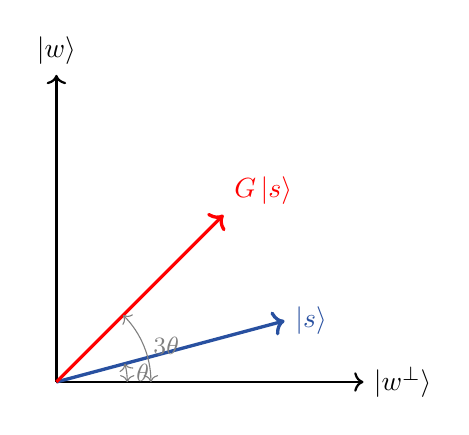
\begin{tikzpicture}[scale=3]
    % axes
    \draw[->, thick] (0,0) -- (1.3,0) node[right] {$\ket{w^\perp}$};
    \draw[->, thick] (0,0) -- (0,1.3) node[above] {$\ket{w}$};

    % initial state
    \draw[->, very thick, circuitblue] (0,0) -- ({cos(15)},{sin(15)}) node[right] {$\ket{s}$};

    % after one iteration
    \draw[->, very thick, red] (0,0) -- ({cos(45)},{sin(45)}) node[above right] {$G\ket{s}$};

    % angles
    \draw[<->, gray] (0.3,0) arc (0:15:0.3) node[midway, right, font=\small] {$\theta$};
    \draw[<->, gray] (0.4,0) arc (0:45:0.4) node[midway, right, font=\small] {$3\theta$};
\end{tikzpicture}
\end{center}

each grover iteration (oracle + diffusion) is a rotation by $2\theta$ in this 2D plane:
\[
G\ket{s} = \sin(3\theta)\ket{w} + \cos(3\theta)\ket{w^\perp}
\]

after $k$ iterations:
\[
G^k\ket{s} = \sin((2k+1)\theta)\ket{w} + \cos((2k+1)\theta)\ket{w^\perp}
\]

we want the amplitude of $\ket{w}$ to be close to 1, which happens when $(2k+1)\theta \approx \pi/2$:
\[
\boxed{k \approx \frac{\pi}{4\theta} \approx \frac{\pi}{4}\sqrt{N}}
\]

\begin{keypoint}
grover's algorithm is a rotation in a 2D plane. each iteration rotates by $2\theta \approx 2/\sqrt{N}$ towards the solution. after $\pi/(4\theta) \approx (\pi/4)\sqrt{N}$ rotations, the state is nearly aligned with $\ket{w}$, and measurement gives the solution with high probability.

if u iterate too many times, u ``overshoot'' and the probability \textbf{decreases}. this is unlike classical search where more iterations always help. u need to know (or estimate) the right number of iterations.
\end{keypoint}

\subsection{Multiple Solutions}

for $M$ solutions out of $N$:
\[
\theta = \arcsin\sqrt{M/N}
\]

number of iterations: $k \approx \frac{\pi}{4}\sqrt{N/M}$

\begin{example}
$N = 1024$, $M = 4$ solutions.

$\theta = \arcsin(2/32) = \arcsin(1/16) \approx 0.0625$

$k \approx \frac{\pi}{4}\sqrt{256} = \frac{\pi}{4} \cdot 16 \approx 12.6$

so approximately 13 iterations.
\end{example}

\subsection{Grover's Optimality}

\begin{keypoint}
\textbf{grover's algorithm is optimal} for unstructured search. the BBBV theorem (Bennett, Bernstein, Brassard, Vazirani, 1997) proves that any quantum algorithm for unstructured search requires $\Omega(\sqrt{N})$ queries. u cant do better than grover's.

this means quantum computers give a \textbf{quadratic} speedup for unstructured search, not exponential. the exponential speedups (like shor's) require \textbf{structure} in the problem (e.g., periodicity, group structure).
\end{keypoint}

\subsection{Grover Worked Example}

\begin{example}
$N = 4$ (2 qubits), searching for $\ket{w} = \ket{11}$.

$\theta = \arcsin(1/2) = \pi/6$. number of iterations: $(2k+1)\pi/6 = \pi/2 \Rightarrow k = 1$.

\textbf{initialize:}
\[
\ket{s} = H^{\otimes 2}\ket{00} = \frac{1}{2}(\ket{00} + \ket{01} + \ket{10} + \ket{11})
\]

\textbf{oracle} (flip phase of $\ket{11}$):
\[
O_f\ket{s} = \frac{1}{2}(\ket{00} + \ket{01} + \ket{10} - \ket{11})
\]

the oracle circuit for marking $\ket{11}$:
\begin{center}
\begin{quantikz}
& \ctrl{1} & \qw \\
& \ctrl{0} & \qw
\end{quantikz}
$= $ CZ gate
\end{center}

\textbf{diffusion operator} $D = 2\ket{s}\bra{s} - I$:

$\ket{s}\bra{s} = \frac{1}{4}\begin{pmatrix} 1 & 1 & 1 & 1 \\ 1 & 1 & 1 & 1 \\ 1 & 1 & 1 & 1 \\ 1 & 1 & 1 & 1 \end{pmatrix}$

$D = 2\ket{s}\bra{s} - I = \frac{1}{2}\begin{pmatrix} -1 & 1 & 1 & 1 \\ 1 & -1 & 1 & 1 \\ 1 & 1 & -1 & 1 \\ 1 & 1 & 1 & -1 \end{pmatrix}$

$D \cdot O_f\ket{s} = \frac{1}{2}\begin{pmatrix} -1 & 1 & 1 & 1 \\ 1 & -1 & 1 & 1 \\ 1 & 1 & -1 & 1 \\ 1 & 1 & 1 & -1 \end{pmatrix} \frac{1}{2}\begin{pmatrix} 1 \\ 1 \\ 1 \\ -1 \end{pmatrix} = \frac{1}{4}\begin{pmatrix} 0 \\ 0 \\ 0 \\ 4 \end{pmatrix} = \begin{pmatrix} 0 \\ 0 \\ 0 \\ 1 \end{pmatrix} = \ket{11}$

after one iteration, the state is exactly $\ket{11}$. measure and get the solution with probability 1.
\end{example}

\subsection{Amplitude Amplification}

grover's algorithm is a special case of the more general \textbf{amplitude amplification} technique.

\begin{definition}
given any quantum algorithm $\mathcal{A}$ that produces the correct answer with probability $p$, amplitude amplification can boost the success probability to near 1 using $O(1/\sqrt{p})$ repetitions of $\mathcal{A}$ and $\mathcal{A}^{-1}$.
\end{definition}

\begin{intuition}
amplitude amplification is to grover's search what the abstract fourier transform is to the FFT --- its the general principle behind the specific algorithm. in grover's, the ``algorithm'' $\mathcal{A}$ is just creating a uniform superposition (hadamard), and the ``correct answer'' is the marked item. but amplitude amplification works with any starting algorithm, making it useful in many QML contexts where u have a quantum subroutine that succeeds with some probability and u want to boost it.
\end{intuition}

%% ========================================================
\section{Quantum Speedups: Quadratic vs Exponential}
%% ========================================================

\begin{keypoint}
its important to understand the diff types of quantum speedups:

\textbf{exponential speedups} (like shor's): require specific mathematical structure in the problem. not generic --- u cant get an exponential speedup for arbitrary problems.

\textbf{quadratic speedups} (like grover's): more broadly applicable but less dramatic. $\sqrt{N}$ instead of $N$ is nice but not world-changing for most practical problem sizes.

\textbf{polynomial speedups}: various algorithms offer speedups that r polynomial but not quite quadratic. often these come with caveats (need QRAM, specific input models, etc.).

for QML: most quantum speedups for machine learning r either quadratic (grover-type) or require specific assumptions abt data access. exponential speedups r rare and usually rely on the data having special structure (like low-rank matrices). this is why the QML advantage question is so nuanced.
\end{keypoint}

\begin{center}
\begin{tikzpicture}[scale=0.7]
    \draw[->] (0,0) -- (9,0) node[right] {$N$ (problem size)};
    \draw[->] (0,0) -- (0,7) node[above] {time / queries};

    % classical brute force
    \draw[thick, red, domain=0.3:6.5, smooth] plot (\x, {0.015*2^(\x)});
    \node[red] at (7.5, 6) {\small $O(2^n)$};

    % grover
    \draw[thick, orange, domain=0.3:8, smooth] plot (\x, {0.12*2^(\x/2)});
    \node[orange] at (8.5, 4) {\small $O(2^{n/2})$};

    % shor
    \draw[thick, circuitblue, domain=0.3:8, smooth] plot (\x, {0.03*\x*\x*\x});
    \node[circuitblue] at (8.5, 1.8) {\small $O(n^3)$};

    % labels
    \node[gray] at (4.5, -0.8) {\small exponential gap (shor) vs quadratic gap (grover)};
\end{tikzpicture}
\end{center}

%% ========================================================
\section{Summary}
%% ========================================================

\begin{keypoint}
the big algorithms:
\begin{enumerate}
    \item \textbf{QFT}: $O(\log^2 N)$ gate complexity, fourier transform over $\mathbb{Z}_N$. cant be used standalone bcs of measurement limitations, but is an essential subroutine
    \item \textbf{QPE}: estimates eigenvalue phases using QFT. foundation for shor's, HHL, quantum chemistry, and many QML algorithms
    \item \textbf{Shor's}: polynomial-time factoring via QPE + order finding. exponential speedup. breaks RSA. uses the structure of modular arithmetic
    \item \textbf{Grover's}: $O(\sqrt{N})$ unstructured search. quadratic speedup, provably optimal. generalizes to amplitude amplification
\end{enumerate}

connection to QML: QPE connects to quantum kernel estimation and quantum principal component analysis. amplitude amplification can boost the success probability of quantum classifiers. the QFT shows up in feature maps for quantum machine learning. shor's is less directly relevant to QML but demonstrates the kind of structure quantum computers exploit.
\end{keypoint}

\end{document}
